\documentclass{article}

\usepackage[a4paper, lmargin=1.25in, rmargin=1.25in, tmargin=1in, bmargin=1in]{geometry}
\usepackage{amsmath}
\usepackage{booktabs}
% \usepackage{xeCJK}
% \setCJKmainfont{宋体}
\usepackage{graphicx}
\graphicspath{ {./fig} }

\usepackage{listings}
\usepackage{color}

\definecolor{dkgreen}{rgb}{0,0.6,0}
\definecolor{gray}{rgb}{0.5,0.5,0.5}
\definecolor{mauve}{rgb}{0.58,0,0.82}

\lstset{
  frame=tb,
  language=R,
  aboveskip=3mm,
  belowskip=3mm,
  showstringspaces=false,
  columns=flexible,
  basicstyle={\small\ttfamily},
  numbers=left,
  numberstyle=\tiny\color{gray},
  keywordstyle=\color{blue},
  commentstyle=\color{dkgreen},
  stringstyle=\color{mauve},
  breaklines=true,
  breakatwhitespace=true,
  tabsize=2
}

\usepackage[hidelinks]{hyperref}
\usepackage{caption}
\usepackage{subcaption}
\usepackage{siunitx}

% \setlength{\parskip}{0.5em}

\title{\textbf{Work Log}}
\author{Liu Yanpei \\ \href{mailto:elliott_liu@outlook.com}{\texttt{elliott\_liu@outlook.com}}}
\date{\today}

\begin{document}
\maketitle
% \tableofcontents
% \newpage

\section*{Hands-on GCN with the Karate Club Dataset}
\addcontentsline{toc}{section}{Hands-on GCN with the Karate Club Dataset}
\stepcounter{section}

\subsection*{Dataset}
% insert dataset image
\begin{figure}[h]
  \centering
  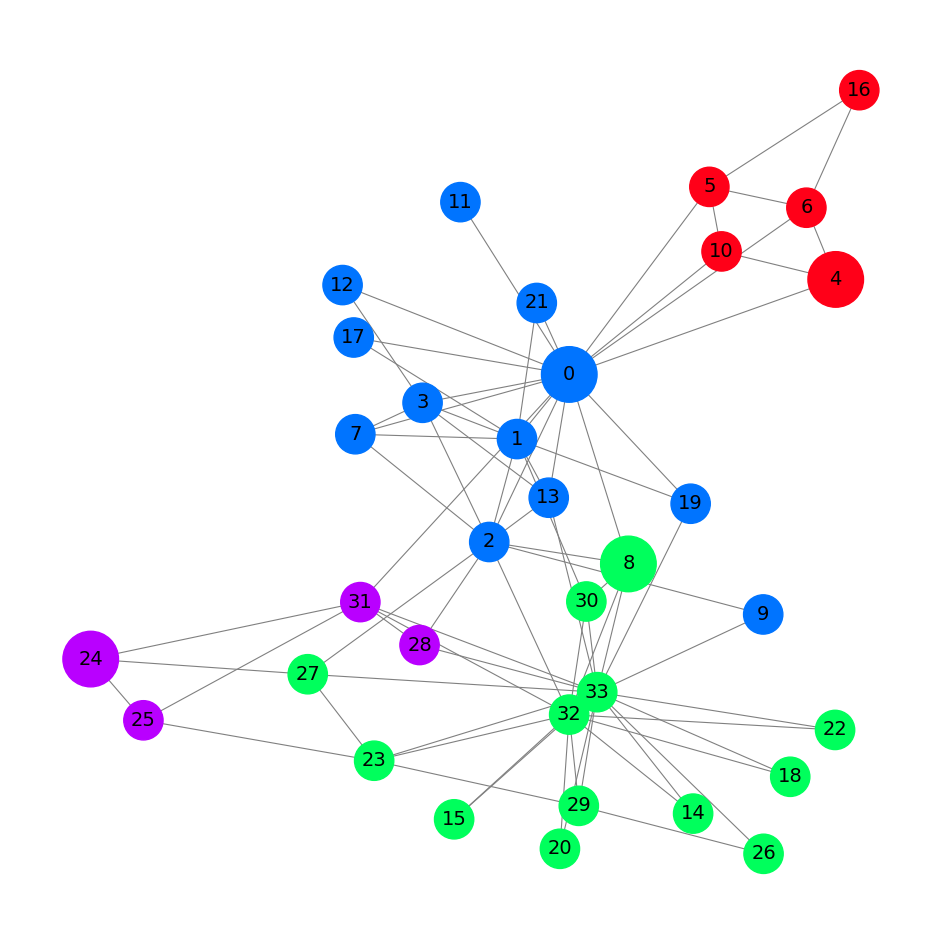
\includegraphics[width=0.5\textwidth]{karateclub.png}
  \caption{Karate Club Network}
  \label{fig:karate}
\end{figure}

\subsection*{GCN formulation}
Here, GCN tries to learn the following mapping
\[f:\mathcal{G}(V,E)\times\mathcal{X}^{|V|\times d}\rightarrow\mathcal{Y},\]
where the graph structure is given by edge index (adjacency list, or less efficiently, adjacency matrix), and the node features are given by a matrix as always.

When it comes to train-test split for semi-supervised learning, the graph structure is kept as a whole and the technique of \texttt{train\_mask} comes as a handy tool for the feature matrix.

I find the following equations comes as fundamental to GCNs:
\[
h_i = \sum_{j\in\tilde{\mathcal{N}_i}}\frac{1}{\sqrt{\deg(i)} \sqrt{\deg(j)}} {W}^T x_j.
\]
Using matrix notations, we have
\[
H^{(l+1)} = \sigma(\hat{A}H^{(l)}W^{(l)}),
\]
where $\hat{A} = {D}^{-\frac{1}{2}}(A + I){D}^{-\frac{1}{2}}$ is the normalized adjacency matrix, and $W^{(l)}$ is of dimension $C^{(l)}\times C^{(l+1)}$. Note that how differnt nodes are sharing the same weight matrix. (\emph{Question: I guess this is different from the lecture, where the weight matrix is different for the node itself and its neighbors? Are there any advantages?})

\subsection*{Caveat: default feature matrix}
In this problem setting, only the graph structure is used for inference and no predefined node features are given or used. Therefore, in that no information is used from the feature space, why not use a simple feature matrix, as simple as an all-ones vector in the length of $|V|$? (Above anything else, it turned out that an all-zeros vector would not work as it leads to zero gradients.)

The resulting performance was outrageously poor and unfortunately it was after a while when I found out the reason to be the poorly designed feature matrix. Looking back at the equations of GCN, it becomes kind of obvious that with this all-ones feature vector, the model is not able to distinguish between different nodes and the information contained in the graph is reduced to only the degrees of nodes. Instead of this choice, an identity matrix which one-hot encodes the nodes would solve the problem.

\subsection*{Performance}
% insert to images of loss and accuracy
\begin{figure}[h]
  \centering
  \begin{subfigure}{0.45\textwidth}
    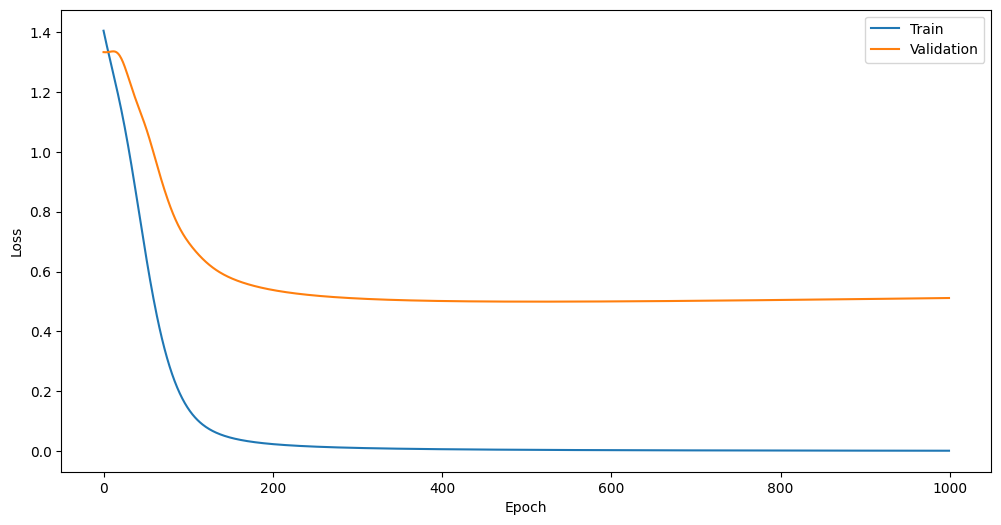
\includegraphics[width=\textwidth]{loss.png}
    \caption{Loss}
  \end{subfigure}
  \begin{subfigure}{0.45\textwidth}
    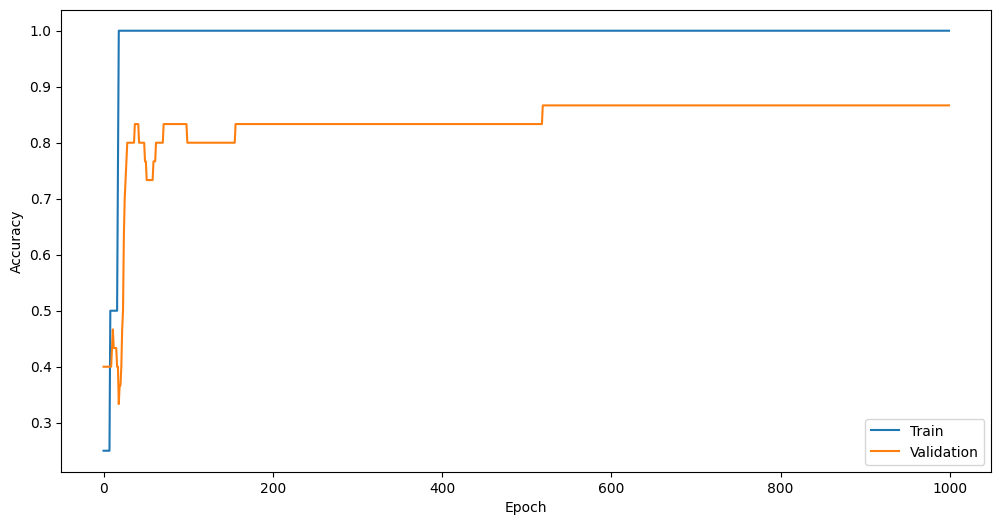
\includegraphics[width=\textwidth]{acc}
    \caption{Accuracy}
  \end{subfigure}
  \caption{Training Loss and Accuracy}
  \label{fig:perf}
\end{figure}

\newpage
\section*{Neural Enhanced Belief Propagation}
\addcontentsline{toc}{section}{Neural Enhanced Belief Propagation}
\stepcounter{section}

\subsection*{Introduction and background}
\begin{itemize}
  \item \textbf{Motivation:} The author suggests two cons of traditional BP. First, in real world scenarios, we may only have access to a poor approximation of the true distribution of the graphical model, leading to suboptimal estimates. Second, BP is not guaranteed to converge in loopy graphs.
  \item \textbf{Error correction decoding algorithm LDPC:}
  \[P(\mathbf{x}) \propto \prod_{s} \left[ \sum_{\substack{n \in N(s)}} x_n = 0 \mod 2 \right] = \prod_{s} f_s(\mathbf{x}_s),\]
  \[P(\mathbf{r}|\mathbf{x}) = \prod_{n} P(r_n | x_n),\]
  \[P(\mathbf{x} | \mathbf{r}) \propto P(\mathbf{x}) P(\mathbf{r} | \mathbf{x}).\]
  \begin{figure}[htb]
    \centering
    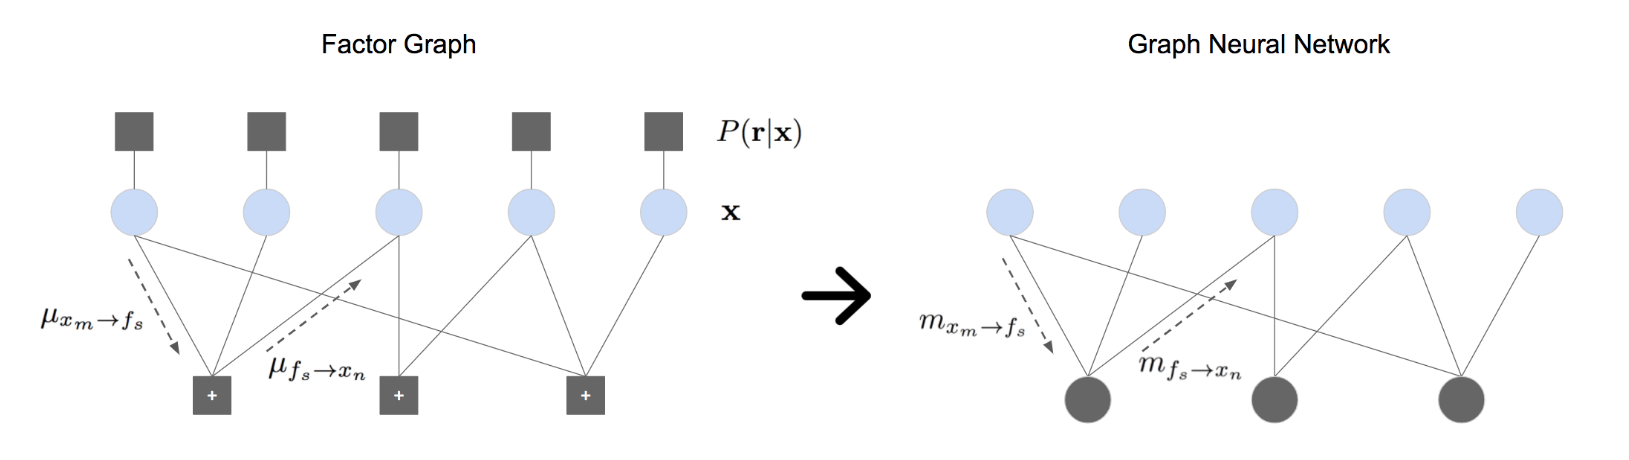
\includegraphics[width=0.95\textwidth]{FGGNN_illustration.png}
    \caption{Illustration of the FG-GNN and LDPC}
    \label{fig:fggnn}
  \end{figure}

  To associate belief propagation with LDPC, it is helpful to think of any factor graphs as a bipartite graph.

  \emph{Question: When we talk about i.i.d. noises (the second equation above), what are we actually referring to?}
  \item
  \textbf{Belief Propagation formulation:}\\
  Variable to factor message:
  \[\mu_{x_m \rightarrow f_s}(x_m) = \prod_{l \in N(x_m) \setminus \{f_s\}} \mu_{f_l \rightarrow x_m}(x_m);\]
  Factor to variable message:
  \[\mu_{f_s \rightarrow x_n}(x_n) = \sum_{x_s \setminus x_n} f_s(x_s) \prod_{m \in N(f_s) \setminus \{x_n\}} \mu_{x_m \rightarrow f_s}(x_m);
  \]
  Marginal estimate:
  \[p(x_n) \propto \prod_{s \in N(x_n)} \mu_{f_s \rightarrow x_n}(x_n).\]
  \end{itemize}

\newpage
\subsection*{NEBP formulation}
\begin{align*}
  \tilde{\mu}_{f \rightarrow x}, \tilde{\mu}_{x \rightarrow f} &= \text{BP}(\mu_{f \rightarrow x}) \\
  M_{f \rightarrow x}^t &= \text{FG-GNN}(h^t, \tilde{\mu}_{f \rightarrow x}, \tilde{\mu}_{x \rightarrow f}) \\
  \mu_{f \rightarrow x}^{t+1} &= \tilde{\mu}_{f \rightarrow x} \cdot f_s(M_{f \rightarrow x}^t) + f_u(M_{f \rightarrow x}^t)
\end{align*}
\begin{figure}[htb]
  \centering
  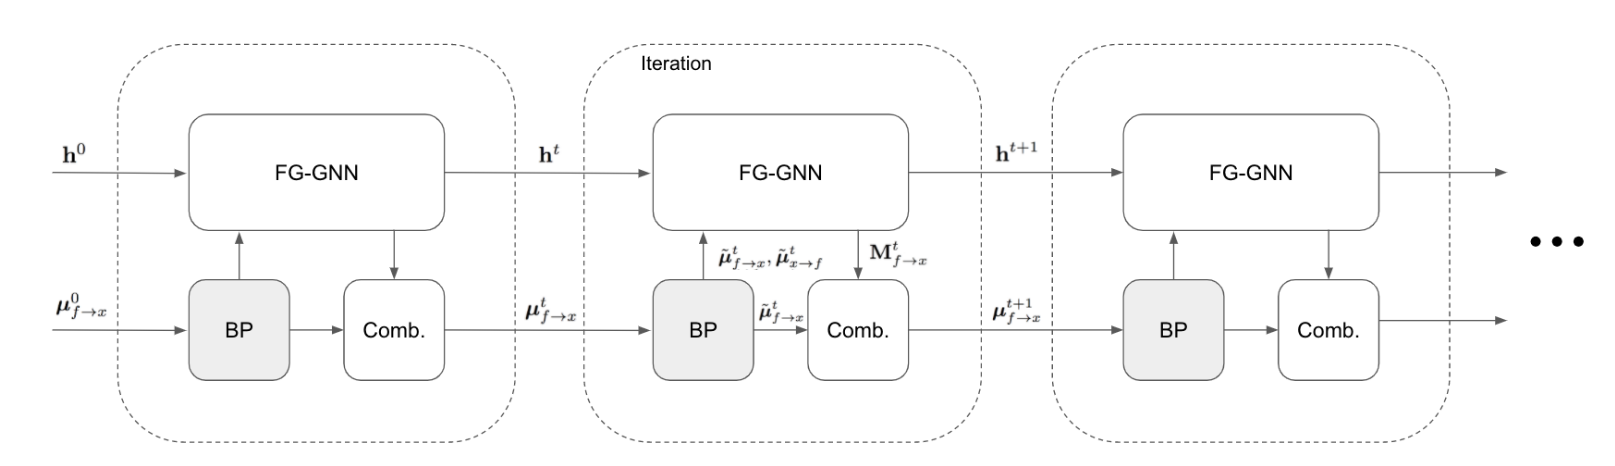
\includegraphics[width=0.95\textwidth]{NEBP_illustration.png}
  \caption{Illustration of the NEBP}
  \label{fig:nebp}
\end{figure}
Many technical details to figure out...
\end{document}